% =============================================================================
% EXERCISE LIST --- MPE assessment style, graduate level (rules/00_estilo_avaliacao.md §8)
% Lecture 1: static games of complete information I --- normal form, dominance,
% dominant-strategy equilibrium, Pareto optimality, IESDS, spatial competition
% (Tadelis 2013, Ch. 3--4; Gibbons 1992, §1.1.A--B and §1.2.A)
%
% TWO MODES (one source file):
%   \solucoesfalse  -> blank LIST (space to solve)
%   \solucoestrue   -> ANSWER KEY + RUBRIC
%
% Compile (copyable PDF, global lmodern+cmap rule):
%   pdflatex lista-lecture-01.tex   (2x) ; check: pdffonts lista-lecture-01.pdf (all Type 1)
% Every result is verified by lista-lecture-01-check.py.
% =============================================================================
\documentclass[11pt,a4paper]{article}
\usepackage[utf8]{inputenc}
\usepackage[T1]{fontenc}
\usepackage{lmodern}   % Type 1 vector fonts (replaces PK bitmaps)
\usepackage{cmap}      % ToUnicode CMap -> copyable text and accents
\usepackage[english]{babel}
\usepackage{amsmath,amssymb,amsfonts,mathtools}
\usepackage[a4paper,margin=2.2cm]{geometry}
\usepackage{enumitem}
\usepackage{fancyhdr}
\usepackage{comment}
\usepackage{xcolor}
\usepackage{microtype}
\usepackage{booktabs}
\usepackage{tikz}

% ====================== CONFIGURATION ======================
\newif\ifsolucoes
\solucoesfalse                 % <<<< \solucoestrue for the ANSWER KEY; \solucoesfalse for the LIST

\newcommand{\disciplina}{Economia das Organizações e dos Incentivos --- MPE Insper}
\newcommand{\listatema}{Lecture 1: Dominance and Iterated Elimination (graduate level)}
\newcommand{\espacoresol}{5cm}   % height of the resolution space in the blank list

% ====================== MACHINERY ======================
\ifsolucoes\includecomment{sol}\else\excludecomment{sol}\fi

\pagestyle{fancy}\fancyhf{}
\lhead{\footnotesize\disciplina}
\rhead{\footnotesize List\ifsolucoes{} --- Answer Key and Rubric\fi}
\cfoot{\footnotesize\thepage}
\renewcommand{\headrulewidth}{0.3pt}
\setlength{\headheight}{14pt}

\setlist{topsep=2pt,itemsep=2pt}
\setlength{\parindent}{0pt}
\newcounter{questao}

\newcommand{\bloco}[3]{\bigskip\noindent
  {\large\bfseries\color{blue!55!black}Block #1 --- #2}\hfill\textit{(#3)}\par
  \noindent\rule{\linewidth}{0.3pt}\smallskip}
\newcommand{\questao}[1]{\refstepcounter{questao}\medskip\noindent
  \textbf{Question \thequestao.}~#1\par}
\newenvironment{alternativas}{\begin{enumerate}[label=\Alph*.,leftmargin=2.2em,topsep=1pt]}{\end{enumerate}}
\newcommand{\gabarito}[1]{\ifsolucoes\par\noindent\textbf{Answer:}~#1\fi}
\newcommand{\resolespaco}{\ifsolucoes\else\par\textit{Resolution:}\vspace{\espacoresol}\par\fi}
\newcommand{\passo}[2]{\par\smallskip\noindent\textbf{Step --- #1.}~#2}
\newcommand{\intuicao}[1]{\par\smallskip\noindent\textit{Economic intuition.}~#1}
\newcommand{\refbib}[1]{\par\smallskip\noindent{\footnotesize\color{black!60}\textbf{Ref:} #1}}
\newcommand{\rubrica}[1]{\par\smallskip\noindent\textbf{Grading rubric.}\begin{itemize}[leftmargin=1.4em,topsep=1pt]#1\end{itemize}}

% =============================================================================
\begin{document}
\begin{center}
  {\Large\bfseries \disciplina}\\[2pt]
  {\large Exercise List: \listatema}\ifsolucoes\\[2pt]\textit{Answer Key and Rubric}\fi
\end{center}
\vspace{2pt}

{\footnotesize\noindent\textbf{Instructions.} Multiple-choice items: mark the single correct
option (no penalty for errors). \emph{True/False} items: every 2 wrong items cancel 1 correct one
(score $=\max\{0,\text{correct}-\text{wrong}/2\}\times$ item value); blank items do not count.
Discursive questions: show every step; a result the item asks you to derive may not be quoted.
All questions are symbolic: state the admissible range of every parameter you use. Throughout,
``dominated'' means dominated by another \emph{pure} strategy, as in Lecture 1; ``IESDS'' removes,
at every round, every strictly dominated strategy of every player. Lecture 2 material (Nash
equilibrium, mixed strategies) is neither needed nor allowed.\par}

% =============================================================================
\bloco{1}{Normal form, dominance and social dilemmas}{Lecture 1 \,\textbullet\, 25 points}

\questao{(10 points) Objective items.}

\textbf{a)} (3 points) \emph{Dominance $\times$ Pareto optimality.} A medical clinic in Recife is
owned by $n\ge2$ partners. Each partner simultaneously either exerts effort ($E$, private cost
$c>0$) or shirks ($S$). If $k$ partners exert effort, the clinic's net revenue is
$Y(k)=yk+\theta\binom{k}{2}$, with $y>0$ and $\theta\ge0$ (every pair of active partners adds
$\theta$ through cross-referrals), and revenue is split equally. The set of costs $c$ for which
shirking is strictly dominant for every partner \emph{and} the resulting profile is Pareto
dominated by some other profile is:
\begin{alternativas}
\item $\big(y/n,\ y\big)$
\item $\big((y+\theta(n-1))/n,\ y+\theta(n-1)/2\big)$
\item $\big((y+\theta(n-1))/n,\ y+\theta(n-1)\big)$
\item $\big(y/n,\ y+\theta(n-1)/2\big)$
\item $\big((y+\theta)/n,\ y+\theta n/2\big)$
\end{alternativas}
\gabarito{B}
\begin{sol}
\passo{marginal return}{Fix the number $k\in\{0,\dots,n-1\}$ of \emph{other} partners who exert
effort. Switching from $S$ to $E$ raises revenue by $Y(k+1)-Y(k)=y+\theta k$, of which the partner
keeps $(y+\theta k)/n$, at cost $c$.}
\passo{dominance}{$S$ strictly dominates $E$ iff $(y+\theta k)/n<c$ for \emph{every}
$k\in\{0,\dots,n-1\}$; since $\theta\ge0$ the binding case is $k=n-1$:
$c>(y+\theta(n-1))/n$. With two strategies, $S$ is then strictly dominant and all-$S$ is the
unique strict dominant-strategy equilibrium, with payoff $0$ for everyone.}
\passo{Pareto}{With $k\ge1$ active partners, the active ones get $Y(k)/n-c$ and the idle ones
$Y(k)/n$. $Y$ is strictly increasing, so $Y(k)/n-c\le Y(n)/n-c$ with equality only at $k=n$. If
$c<Y(n)/n$, all-$E$ gives everyone $Y(n)/n-c>0$: it Pareto dominates all-$S$. If $c\ge Y(n)/n$,
every profile with $k\ge1$ gives each active partner $Y(k)/n-c<0$ for $k<n$, and everyone $\le0$
at $k=n$: no profile Pareto dominates all-$S$. Hence the condition is
$c<Y(n)/n=y+\theta(n-1)/2$.}
\passo{non-empty}{$y+\tfrac{\theta(n-1)}{2}-\tfrac{y+\theta(n-1)}{n}=\tfrac{(n-1)y}{n}+\tfrac{\theta(n-1)(n-2)}{2n}>0$ for $n\ge2$.}
\passo{distractors}{A sets $\theta=0$ in both bounds (the lecture's partnership); D checks
dominance only against $k=0$, where effort pays least (necessary, not sufficient); C compares
with the last partner's marginal revenue instead of per-capita revenue; E counts $\theta$ once per
partner instead of once per pair, in both bounds.}
\intuicao{Synergy makes effort most valuable when everyone else works, so dominance must hold in
that best case; the dilemma needs full cooperation to pay per capita.}
\refbib{Lecture 1, ``Examples'' (partnership); Tadelis (2013) \S4.1.2--4.1.3, pp.~61--62, and
\S3.3.3, p.~56.}
\end{sol}

\medskip
\textbf{b)} (3 points) \emph{Weak dominance $\times$ IESDS.} A court-ordered sale (\emph{leilão
judicial}) of a warehouse in Campinas uses a sealed-bid second-price rule with a public reserve
price $r>0$: $n\ge2$ bidders submit bids $b_j\in[0,\infty)$; if every bid is below $r$ there is no
sale; otherwise the highest bidder wins (ties broken uniformly at random) and pays
$\max\{r,\text{highest other bid}\}$. Bidder $i$ values the warehouse at $v_i>r$. Which statement
is correct?
\begin{alternativas}
\item Bidding $v_i$ strictly dominates every other bid, so IESDS selects truthful bidding for every bidder whose value exceeds $r$.
\item Bidding $v_i$ weakly dominates the bids above $v_i$ only; bids in $[r,v_i)$ are not weakly dominated, since they lower the price paid.
\item Bidding $v_i-r$ weakly dominates every other bid, because the reserve price is a cost that the winner must net out of the value.
\item Bidding $v_i$ weakly dominates every other bid, yet no bid of any bidder is strictly dominated, so IESDS removes no strategy at all.
\item Bidding $v_i$ weakly dominates every other bid, and the bids below $r$ are strictly dominated by $v_i$, so IESDS removes them.
\end{alternativas}
\gabarito{D}
\begin{sol}
\passo{price is not one's own bid}{Let $p\equiv\max\{r,h\}$, $h$ the highest rival bid. A winning
bidder pays $p$, which does not depend on her own bid; her bid only decides \emph{whether} she wins.}
\passo{weak dominance}{If $p<v_i$: bidding $v_i$ wins and earns $v_i-p>0$; any $b>p$ earns the same,
$b<p$ earns $0$, $b=p$ earns at most $v_i-p$. If $p>v_i$: $v_i$ loses (0); any winning bid pays
$p>v_i$ (negative). If $p=v_i$: every bid earns $0$. So $v_i$ is never worse, and it is strictly
better against rival bids with $p\in(b,v_i)$ (for $b<v_i$) or with $h\in(v_i,b)$ (for $b>v_i$).}
\passo{no strict dominance}{Take any two bids $b\ne b'$ of any bidder $j$ and the rival profile
in which someone bids above $\max\{b,b'\}$: both earn $0$. No inequality is strict for all rival
profiles, so no bid is strictly dominated: $S_j^1=S_j$ and IESDS has no bite.}
\passo{distractors}{A confuses weak with strict dominance; B assumes the bid sets the price;
C subtracts the reserve from the value; E calls the bids below $r$ strictly dominated, but they tie
with $v_i$ whenever a rival bids above $v_i$.}
\intuicao{Truthful bidding is robust (never a mistake), but the argument behind it uses weak
dominance; common knowledge of rationality alone, through IESDS, says nothing in this auction.}
\refbib{Tadelis (2013) \S13.1.1, pp.~272--273 (Proposition 13.1, no reserve); Lecture 1,
``Examples'' (second-price auction) and ``Dominance''.}
\end{sol}

\medskip
\textbf{c)} (2 points, T or F) \emph{Invariance $\times$ dominance.} Let $G$ be a finite game with a
strict dominant-strategy equilibrium $s^D$. Then there is $\varepsilon>0$ such that $s^D$ is a strict
dominant-strategy equilibrium of every game $G'$ with the same players and strategy sets whose payoffs
satisfy $|u_i'(s)-u_i(s)|<\varepsilon$ for every $i$ and every $s$.
\gabarito{T}
\begin{sol}
\passo{proof}{Let $g\equiv\min\{u_i(s_i^D,s_{-i})-u_i(s_i,s_{-i}):\ i\in I,\ s_i\ne s_i^D,\ s_{-i}\in S_{-i}\}$,
a minimum over a finite set of strictly positive numbers, so $g>0$. Take $\varepsilon=g/2$. Then
$u_i'(s_i^D,s_{-i})-u_i'(s_i,s_{-i})>g-2\varepsilon=0$ for every $i$, $s_i\ne s_i^D$, $s_{-i}$.}
\passo{what breaks it}{Finiteness: with infinite strategy sets the infimum gap can be $0$ (in
Question 2 the gap is $\tfrac c2(e_i-e_i^D)^2$). Strictness: if $U$ weakly dominates $D$ with
$u_1(U,L)=u_1(D,L)$, raising $u_1(D,L)$ by $\varepsilon/2$ destroys the weak dominance for every
$\varepsilon>0$.}
\refbib{Tadelis (2013) \S3.3.2, pp.~55--56 (invariance); \S4.1.3, p.~62.}
\end{sol}

\medskip
\textbf{d)} (2 points, T or F) \emph{Pareto optimality $\times$ dominance.} In every finite game,
with any number of players, that has a strict dominant-strategy equilibrium $s^D$, every profile that
Pareto dominates $s^D$ has \emph{every} player $i$ using a strategy different from $s_i^D$.
\gabarito{F}
\begin{sol}
\passo{true for two players}{If $s'$ Pareto dominates $s^D$ and $s'_1=s^D_1$, then $s'_2\ne s^D_2$
and $u_2(s')=u_2(s_1^D,s_2')<u_2(s^D)$ by strict dominance: contradiction. Symmetrically for player 2.}
\passo{counterexample with three players}{Players 1 and 2 play a prisoner's dilemma whose payoffs do
not depend on player 3: $(M,M)\mapsto(-1,-1)$, $(M,F)\mapsto(-4,0)$, $(F,M)\mapsto(0,-4)$,
$(F,F)\mapsto(-3,-3)$. Player 3 chooses $X$ or $Y$ with $u_3=u_1+u_2+\mathbb 1\{s_3=X\}$, so $X$ is
strictly dominant and $s^D=(F,F,X)$. The profile $(M,M,X)$ gives $(-1,-1,-1)$ against
$(-3,-3,-5)$: it Pareto dominates $s^D$ while player 3 keeps $X$. With $n\ge3$ a player who does
not deviate can gain from the others' deviations.}
\refbib{Lecture 1, ``Dominance and social dilemmas''; Tadelis (2013) \S4.1.3, p.~62.}
\end{sol}

% -----------------------------------------------------------------------------
\questao{(15 points) \emph{Dominance $\times$ Pareto optimality and social dilemmas $\times$
solution-concept criteria.} An accounting firm in Belo Horizonte is a partnership of $n\ge2$
partners. Simultaneously, each partner $i$ chooses an effort level $e_i\ge0$. Firm revenue is
$y\sum_{j}e_j$ ($y>0$); partner $i$ bears the private cost $\tfrac c2e_i^2$ ($c>0$) and receives the
share $\alpha_i\ge0$ of revenue, with $\sum_i\alpha_i=1$ fixed in the partnership agreement. Efforts
are not observable by the other partners, so nothing else can be contracted on; each partner cares
only about her own payoff. Unless stated otherwise, $\alpha_i=1/n$.}

\textbf{a)} (3 points) Write the game in normal form $G=(I,\{S_i\},\{u_i\})$. Prove that every
partner has a strictly dominant strategy, for any shares $(\alpha_i)$, and find it. Draw, in the
$(e_i,u_i)$ plane, partner $i$'s payoff as a function of her own effort for two different values of
the others' total effort, and read the dominance property off the figure.
\resolespaco
\begin{sol}
\passo{normal form}{$I=\{1,\dots,n\}$, $S_i=[0,\infty)$, and
$$u_i(e)=\alpha_iy\sum_je_j-\tfrac c2e_i^2=\underbrace{\alpha_iy\textstyle\sum_{j\ne i}e_j}_{\text{others}}+\alpha_iye_i-\tfrac c2e_i^2.$$}
\passo{dominance}{Let $e_i^D\equiv\alpha_iy/c$. For any $e_i$ and any $e_{-i}$,
$$u_i(e_i^D,e_{-i})-u_i(e_i,e_{-i})=\alpha_iy(e_i^D-e_i)-\tfrac c2\big((e_i^D)^2-e_i^2\big)
=\tfrac c2\,(e_i-e_i^D)^2,$$
using $\alpha_iy=ce_i^D$. The difference does not depend on $e_{-i}$ and is strictly positive for
$e_i\ne e_i^D$: $e_i^D$ is strictly dominant (with $\alpha_i=0$ it is $e_i^D=0$).}
\passo{graph}{The others' effort enters additively, so a change in $E_{-i}=\sum_{j\ne i}e_j$ shifts
the whole parabola vertically by $\alpha_iy\,\Delta E_{-i}$ (gray arrow) without moving its peak.}
\begin{center}
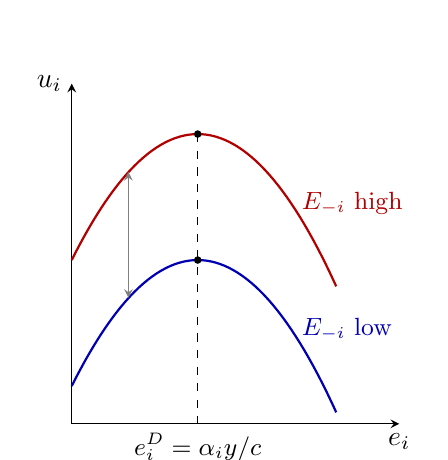
\begin{tikzpicture}[scale=1.6,>=stealth]
  \draw[->] (0,0) -- (2.6,0) node[below] {$e_i$};
  \draw[->] (0,0) -- (0,2.7) node[left] {$u_i$};
  \draw[thick,blue!70!black,domain=0:2.1,samples=60] plot (\x,{0.3+2*\x-\x*\x});
  \draw[thick,red!70!black,domain=0:2.1,samples=60] plot (\x,{1.3+2*\x-\x*\x});
  \node[blue!70!black,right] at (1.75,0.75) {\small $E_{-i}$ low};
  \node[red!70!black,right] at (1.75,1.75) {\small $E_{-i}$ high};
  \draw[dashed] (1,2.3) -- (1,0) node[below] {\small $e_i^D=\alpha_iy/c$};
  \fill (1,1.3) circle (0.03); \fill (1,2.3) circle (0.03);
  \draw[<->,gray] (0.45,1.0) -- (0.45,2.0);
\end{tikzpicture}
\end{center}
\passo{reading}{Whatever partner $i$ believes about the others, her payoff curve peaks at the same
$e_i^D$: the ranking of her own strategies is belief-free, which is what dominance means.}
\refbib{Tadelis (2013) \S3.1, pp.~46--49; \S4.1.1--4.1.2, pp.~60--61.}
\rubrica{
\item Normal form with $S_i$ and $u_i$: 0.5 pt.
\item Dominance proved for \emph{every} $e_{-i}$ (difference identity or equivalent): 1.25 pts. Only
  the first-order condition $\alpha_iy=ce_i$ (best reply, not dominance): max.\ 1 pt on the item.
\item Graph: labelled axes 0.25, two parabolas with the same peak 0.5, vertical shift labelled 0.25;
  reading 0.25. A graph contradicting the algebra loses the graph points.
}
\end{sol}

\textbf{b)} (3 points) Take equal shares. Show that the game has a unique strict dominant-strategy
equilibrium and a unique iterated-elimination equilibrium. Prove that this profile is Pareto
dominated, and find the set of symmetric effort levels $\bar e$ such that $(\bar e,\dots,\bar e)$
Pareto dominates it. Which symmetric profile is best for every partner?
\resolespaco
\begin{sol}
\passo{equilibrium}{From a), $e^D=y/(nc)$ for everyone. A strict dominant-strategy equilibrium is
unique (Lecture 1 proposition), and in round 1 of IESDS every $e_i\ne e^D$ is strictly dominated by
$e^D$, so $S_i^1=\{e^D\}$: the unique iterated-elimination equilibrium.}
\passo{symmetric payoffs}{In $(\bar e,\dots,\bar e)$ each partner receives $\tfrac1n\,y\,n\bar e$
and pays $\tfrac c2\bar e^2$: $u(\bar e)=y\bar e-\tfrac c2\bar e^2$. At $e^D$:
$u^D=\dfrac{y^2}{nc}-\dfrac{y^2}{2n^2c}=\dfrac{y^2(2n-1)}{2n^2c}$.}
\passo{dominating set}{$u(\bar e)>u^D\iff\tfrac c2\bar e^2-y\bar e+u^D<0$. The discriminant is
$y^2-2cu^D=y^2(n-1)^2/n^2>0$ for $n\ge2$, with roots $\tfrac yc\big(1\pm\tfrac{n-1}n\big)$:
$$\bar e\in\Big(\frac{y}{nc},\ \frac{(2n-1)\,y}{nc}\Big).$$
All partners gain in the same proportion, so these are exactly the symmetric Pareto improvements.}
\passo{best symmetric profile}{$u(\bar e)$ is maximized at $\bar e=y/c\equiv e^*$, the midpoint of
the interval, with $u=y^2/(2c)$. It is Pareto optimal: $\sum_iu_i=y\sum_je_j-\tfrac c2\sum_je_j^2$
(shares sum to 1) is maximized at $e_j=y/c$ for all $j$, and any Pareto improvement would raise the sum.}
\intuicao{Each partner keeps $1/n$ of the value of her effort but bears all of its cost: individually
dominant, collectively dominated. This is the prisoner's dilemma with a continuum of strategies.}
\refbib{Lecture 1, ``Dominance and social dilemmas''; Tadelis (2013) \S4.1.3, p.~62; M\&R Ch.~2,
``Efficiency'', pp.~22--24.}
\rubrica{
\item $e^D$ and both uniqueness claims (strict DSE and round-1 IESDS): 0.75 pt.
\item $u^D$: 0.5 pt. Dominating interval with both roots: 1 pt.
\item $e^*=y/c$ and its Pareto optimality argued: 0.75 pt.
\item Only $e^*$ shown to dominate (no interval): max.\ 2 pts. Arithmetic slip with right method: $-0.5$ pt.
}
\end{sol}

\textbf{c)} (3 points) Return to general shares. Prove that no sharing rule
($\alpha_i\ge0$, $\sum_i\alpha_i=1$) makes the efficient profile $(y/c,\dots,y/c)$ a dominant-strategy
equilibrium. Characterize the sharing rule that maximizes total surplus $W\equiv\sum_iu_i$ at the
dominant-strategy equilibrium, and the rule that minimizes it.
\resolespaco
\begin{sol}
\passo{impossibility}{From a), $e_i^D=\alpha_iy/c=y/c\iff\alpha_i=1$. Budget balance allows this for
at most one partner, and then $\alpha_j=0$ and $e_j^D=0\ne y/c$ for the other $n-1\ge1$ partners.}
\passo{surplus at the DSE}{With $e_j^D=\alpha_jy/c$: $W(\alpha)=y\sum_je_j^D-\tfrac c2\sum_j(e_j^D)^2
=\dfrac{y^2}{c}\sum_j\big(\alpha_j-\tfrac12\alpha_j^2\big)$.}
\passo{maximization}{$\max W$ s.t.\ $\sum_j\alpha_j=1$, $\alpha_j\ge0$. The objective is a sum of
strictly concave functions. Lagrangian $\sum_j(\alpha_j-\tfrac12\alpha_j^2)-\mu(\sum_j\alpha_j-1)$;
FOC $1-\alpha_j=\mu$ for every $j$ with $\alpha_j>0$, so all positive shares are equal. A zero share
would need $1-0\le\mu=1-\tfrac1{n'}<1$ ($n'$ the number of positive shares): impossible. Hence the
unique maximizer is $\alpha_j=1/n$, with $W=\dfrac{y^2}{c}\Big(1-\dfrac1{2n}\Big)$.}
\passo{minimization}{A concave function on the simplex attains its minimum at a vertex:
$\alpha=(1,0,\dots,0)$, one partner works at $y/c$ and the rest at $0$, $W=y^2/(2c)$.}
\intuicao{Equal split is the best a budget-balanced partnership can do, and it is still inefficient:
the inefficiency comes from budget balance itself, since every partner would need the whole
marginal product, $\sum_i\alpha_i=n$, which only an outside party could fund.}
\refbib{Tadelis (2013) \S3.3.3, p.~56; M\&R Ch.~2, ``Efficiency'', pp.~22--24.}
\rubrica{
\item Impossibility with the budget-balance argument: 1 pt.
\item $W(\alpha)$: 0.5 pt. Equal split proved optimal (concavity + FOC, corners excluded): 1 pt.
\item Minimum at a vertex: 0.5 pt.
\item Equal split asserted ``by symmetry'' without proof: 0 for that line.
}
\end{sol}

\textbf{d)} (3 points) With equal shares, quantify the social dilemma: total surplus at the
efficient profile, $W^*$, and at the dominant-strategy equilibrium, $W^D$; the relative loss
$L/W^*$, where $L\equiv W^*-W^D$; the payoff gap per partner; and the effort ratio $e^D/e^*$.
\resolespaco
\begin{sol}
\passo{levels}{$W^*=n\,u(e^*)=\dfrac{ny^2}{2c}$; $W^D=n\,u^D=\dfrac{y^2(2n-1)}{2nc}$.}
\passo{loss}{$\dfrac{L}{W^*}=1-\dfrac{2n-1}{n^2}=\dfrac{(n-1)^2}{n^2}$; per partner,
$u(e^*)-u^D=\dfrac{y^2(n-1)^2}{2n^2c}$; effort ratio $e^D/e^*=1/n$.}
\passo{benchmark}{$n=2$: a quarter of the surplus is lost; $n=5$: $64\%$.}
\intuicao{Effort falls to $1/n$ of its efficient level, and the surplus loss is quadratic in the
shortfall: the dilemma deepens fast with the number of partners.}
\refbib{Lecture 1, ``Dominance and social dilemmas''; Tadelis (2013) \S3.3.3, p.~56.}
\rubrica{
\item $W^*$ and $W^D$: 1.25 pts. $L/W^*$ simplified: 1 pt. Gap and ratio: 0.75 pt.
\item $W^D$ computed with the efficient effort for one partner and $e^D$ for the others: max.\ 1 pt.
}
\end{sol}

\textbf{e)} (3 points) Parameter analysis. Prove the sign of the effect of $y$, $c$ and $n$
(treated as continuous) on $e^D$, $e^*$, the per-partner payoff $u^D$, total surplus $W^D$ and the
relative loss $L/W^*$. Summarize in a table, study $n\to1$, $n\to\infty$ and $c\to0$, and give the
economic reading.
\resolespaco
\begin{sol}
\passo{signs}{$e^D=y/(nc)$: $+y$, $-c$, $-n$. $e^*=y/c$: $+y$, $-c$, no $n$.
$u^D=\tfrac{y^2}{c}\tfrac{2n-1}{2n^2}$: $\partial_nu^D=-\dfrac{y^2(n-1)}{n^3c}<0$ for $n>1$.
$W^D=\tfrac{y^2}{c}\big(1-\tfrac1{2n}\big)$: $\partial_nW^D=\dfrac{y^2}{2n^2c}>0$.
$L/W^*=(1-1/n)^2$: $\partial_n=2(n-1)/n^3>0$; no $y$, no $c$.}
\begin{center}
\begin{tabular}{lccc}\toprule
 & $y$ & $c$ & $n$\\\midrule
$e^D$ & $+$ & $-$ & $-$\\
$e^*$ & $+$ & $-$ & $0$\\
$u^D$ & $+$ & $-$ & $-$\\
$W^D$ & $+$ & $-$ & $+$\\
$L/W^*$ & $0$ & $0$ & $+$\\\bottomrule
\end{tabular}
\end{center}
\passo{limits}{$n\to1$: $e^D\to e^*$, $L\to0$ (a sole proprietor faces no dilemma). $n\to\infty$:
$e^D,u^D\to0$, $W^D\to y^2/c$ (bounded) while $W^*\to\infty$, so $L/W^*\to1$. $c\to0$: every level
diverges, $L/W^*$ is unchanged: the loss share is a pure function of $n$.}
\passo{reading}{Productivity and cost scale the stakes but not the distortion; only the number of
claimants on each unit of output does. More partners raise total effort ($W^D$ rises) but lower each
one's effort and payoff. The prediction is invariant in the sense of Lecture 1: small changes in
$y$ or $c$ move $e^D$ continuously, and the dominance argument never uses beliefs.}
\rubrica{
\item Signs proved: 1.5 pts (the $W^D$-in-$n$ sign, opposite to $u^D$, counts 0.5).
\item Table 0.25 pt; limits 0.5 pt; reading 0.75 pt.
\item Signs listed without proof or reading: max.\ half the item.
}
\end{sol}

% =============================================================================
\bloco{2}{Iterated elimination of strictly dominated strategies}{Lecture 1 \,\textbullet\, 25 points}

\questao{(10 points) Objective items.}

\textbf{a)} (3 points) \emph{IESDS $\times$ common knowledge of rationality.} A distributor
(player 1, rows) and a retailer (player 2, columns) in the Zona Franca de Manaus play the game below,
in which $x\in\mathbb R$ is the distributor's payoff at $(U,C)$:
$$\begin{array}{c|ccc}
 & L & C & R\\\hline
U & 2,3 & x,2 & 5,0\\
M & 5,3 & 4,4 & 2,2\\
D & 1,4 & 1,5 & 4,6
\end{array}$$
IESDS selects a unique profile if and only if, and the number of rounds it takes is:
\begin{alternativas}
\item $x>1$; four rounds
\item $x>1$; three rounds
\item $1<x<4$; three rounds
\item $x<4$; two rounds
\item $1<x<4$; four rounds
\end{alternativas}
\gabarito{E}
\begin{sol}
\passo{round 1}{$U$ vs $D$ column by column: $2>1$, $x$ against $1$, $5>4$; so $U$ strictly
dominates $D$ iff $x>1$. $M$ does not
dominate $D$ ($2<4$ at $R$). Player 2: no column dominates another ($L$ is best against $U$, $R$
against $D$, and $C$ beats $L$ at $M$). If $x\le1$ nothing is removed and $S^\infty=S$.}
\passo{round 2 ($x>1$)}{Rows $\{U,M\}$: $R$ gives $(0,2)$, strictly below $L$ $(3,3)$: $R$ removed.
$U$ vs $M$ still compares column $R$ ($5>2$): nothing removed for player 1.}
\passo{round 3}{Columns $\{L,C\}$: $M$ $(5,4)$ strictly dominates $U$ $(2,x)$ iff $x<4$.}
\passo{round 4}{Row $M$: $C$ $(4)>L$ $(3)$; the survivor is $(M,C)$. If $x\ge4$ the process stops at
$\{U,M\}\times\{L,C\}$. So: unique iff $1<x<4$, after four rounds; the last round uses third-order
knowledge of rationality.}
\passo{distractors}{A and B drop the condition $x<4$; C and D miscount rounds (C also merges rounds 2
and 3, which are sequential because $U$ vs $M$ hinges on column $R$); D also drops $x>1$.}
\refbib{Tadelis (2013) \S4.2.1, pp.~63--65; Gibbons (1992) \S1.1.B, pp.~4--8.}
\end{sol}

\medskip
\textbf{b)} (3 points) \emph{Weak dominance $\times$ order of elimination.} In the game below,
consider iterated elimination of \emph{weakly} dominated strategies, removing one strategy at a time
in any order until no strategy is weakly dominated:
$$\begin{array}{c|ccc}
 & L & C & R\\\hline
U & 1,2 & 1,0 & 0,1\\
M & 1,2 & 2,2 & 2,1\\
D & 0,0 & 2,1 & 1,2
\end{array}$$
Which statement is correct?
\begin{alternativas}
\item Some orders end at the single profile $(M,L)$ and others at the single profile $(M,C)$, so player 1's final payoff (1 or 2) depends on the order.
\item Every order ends at $(M,C)$, because $M$ weakly dominates both $U$ and $D$, after which player 2 prefers $C$.
\item IESDS (strict) already selects $(M,C)$, and every order of weak elimination agrees with it.
\item Removing all weakly dominated strategies at once in every round ends at the single profile $(M,C)$.
\item Some orders end at $(M,L)$ and others at $(U,L)$, so player 1's final payoff is $1$ in every order.
\end{alternativas}
\gabarito{A}
\begin{sol}
\passo{strict}{No strategy is strictly dominated ($U$ ties $M$ at $L$, $D$ ties $M$ at $C$; no column
is dominated), so IESDS removes nothing: C is false.}
\passo{weak, first step}{$M$ weakly dominates $U$ (tie at $L$) and $D$ (tie at $C$); no column is
weakly dominated in the full game.}
\passo{order 1}{Remove $U$; on rows $\{M,D\}$, $C$ $(2,1)$ weakly dominates $L$ $(2,0)$: remove $L$;
on columns $\{C,R\}$, $M$ $(2,2)$ weakly dominates $D$ $(2,1)$: remove $D$; then $R$ $(1)<C$ $(2)$:
end at $(M,C)$, payoffs $(2,2)$.}
\passo{order 2}{Remove $D$; on rows $\{U,M\}$, $L$ $(2,2)$ weakly dominates $C$ $(0,2)$: remove $C$;
on columns $\{L,R\}$, $M$ $(1,2)$ weakly dominates $U$ $(1,0)$: remove $U$; then $R$ $(1)<L$ $(2)$:
end at $(M,L)$, payoffs $(1,2)$.}
\passo{other claims}{All at once: round 1 removes $U$ and $D$; then $R$; $L$ and $C$ tie for player
2: $\{M\}\times\{L,C\}$, not a singleton (D false). $M$ is never removed, and a run that keeps $U$
ends at $\{U,M\}\times\{L\}$, never at the single profile $(U,L)$ (E false); B is refuted by order 2.}
\intuicao{A weakly dominated strategy can be the only reason another strategy is weakly dominated;
removing it first changes what is removed later. Strict dominance does not have this problem
(item d).}
\refbib{Tadelis (2013) \S4.1.3, pp.~62--63; Lecture 1, ``Dominance'' (weak dominance).}
\end{sol}

\medskip
\textbf{c)} (2 points, T or F) \emph{IESDS $\times$ existence.} In every normal-form game, IESDS
leaves every player at least one strategy: $S_i^\infty\ne\varnothing$ for every $i$.
\gabarito{F}
\begin{sol}
\passo{counterexample}{Let $S_1=[0,1)$ and $u_1(s)=s_1$ (player 2 arbitrary). Every $s_1$ is strictly
dominated by $(1+s_1)/2\in(s_1,1)$, so $S_1^1=\varnothing$ already in round 1.}
\passo{finite games}{With finite sets, the strategy $\hat s_i$ that maximizes
$\sum_{s_{-i}\in S_{-i}^{k-1}}u_i(s_i,s_{-i})$ over $S_i^{k-1}$ cannot be strictly dominated within
$S^{k-1}$ (a dominator would have a strictly larger sum), so $S_i^k\ne\varnothing$, and the process
stops after finitely many rounds. The existence claim of the lecture is a claim about finite games.}
\refbib{Tadelis (2013) \S4.2.3, pp.~67--68; \S3.3.2, p.~55 (existence).}
\end{sol}

\medskip
\textbf{d)} (2 points, T or F) \emph{IESDS $\times$ order of elimination.} In a finite game, removing
at each step \emph{some} (not necessarily all) of the strictly dominated strategies, in any order,
until none is left always ends at the same sets $S_i^\infty$ as the lecture's procedure.
\gabarito{T}
\begin{sol}
\passo{setup}{Let $A$ be the lecture's result and $B$ the end of any other run; both are terminal (no
strictly dominated strategy relative to themselves). Show $B\subseteq A$; $A\subseteq B$ is the same
argument with the roles swapped.}
\passo{proof}{Suppose some strategy of $B$ is removed by the lecture's procedure; let $s_i\in B_i$ be
one removed first, at a round whose current sets contain $B$. It was dominated by some $s_i'$ relative
to a superset of $B_{-i}$, so the set $\mathcal D=\{t\in S_i:\ t\text{ strictly dominates }s_i\text{ on }B_{-i}\}$
is non-empty. Pick $t^*\in\mathcal D$ maximizing $\sum_{s_{-i}\in B_{-i}}u_i(t,s_{-i})$ (finite). If
$t^*\in B_i$, $s_i$ is dominated within $B$: contradiction. If $t^*\notin B_i$, the other run removed
it, dominated by some $t'$ relative to a superset of $B_{-i}$; then $t'$ dominates $s_i$ on $B_{-i}$,
so $t'\in\mathcal D$ with a larger sum: contradiction.}
\refbib{Tadelis (2013) \S4.2.1, pp.~63--65; Gibbons (1992) \S1.1.B, pp.~4--8.}
\end{sol}

% -----------------------------------------------------------------------------
\questao{(15 points) \emph{IESDS $\times$ common knowledge of rationality $\times$ solution-concept
criteria (uniqueness, invariance).} Two cement producers supply a regional market in the North of
Brazil and choose quantities simultaneously. Inverse demand is $P(Q)=\max\{a-bQ,0\}$ with
$Q=q_1+q_2$; firm $i$ has constant marginal cost $c_i\in(0,a)$ and no fixed cost;
$S_i=[0,\infty)$ and $u_i=\pi_i(q_i,q_j)=q_i\big(P(q_i+q_j)-c_i\big)$.}

\textbf{a)} (3 points) Show that, for each $q_j\ge0$, $\pi_i(\cdot,q_j)$ is strictly increasing up to
a unique profit-maximizing quantity $\mathrm{BR}_i(q_j)$ and strictly decreasing beyond it, and find
$\mathrm{BR}_i$. Determine $S_i^1$ exactly, and say where the assumption $c_i>0$ is used.
\resolespaco
\begin{sol}
\passo{two regions}{If $q_i+q_j<a/b$: $\pi_i=q_i(a-c_i-bq_j)-bq_i^2$, with
$\partial\pi_i/\partial q_i=a-c_i-bq_j-2bq_i$, strictly decreasing in $q_i$. If $q_i+q_j\ge a/b$:
$\pi_i=-c_iq_i$, strictly decreasing because $c_i>0$. $\pi_i$ is continuous at the kink.}
\passo{best reply}{Hence $\pi_i(\cdot,q_j)$ rises up to
$\mathrm{BR}_i(q_j)=\max\big\{\tfrac{a-c_i-bq_j}{2b},0\big\}$ and falls strictly afterwards (the
kink lies beyond $\mathrm{BR}_i(q_j)$ since the price there is $0<c_i$). $\mathrm{BR}_i$ is
non-increasing with slope $-\tfrac12$ or $0$.}
\passo{round 1}{$\mathrm{BR}_i(q_j)\le\mathrm{BR}_i(0)=m_i\equiv\tfrac{a-c_i}{2b}$. For $q>m_i$ and
every $q_j$, both $m_i$ and $q$ lie in the decreasing part with $m_i<q$: $\pi_i(m_i,q_j)>\pi_i(q,q_j)$,
so $q$ is strictly dominated by $m_i$. Each $q\in[0,m_i]$ is the \emph{unique} maximizer against
$q_j=(a-c_i-2bq)/b\ge0$, so it cannot be strictly dominated. $S_i^1=[0,m_i]$.}
\passo{role of $c_i>0$}{With $c_i=0$, every $q_i$ earns $0$ against $q_j\ge a/b$, so $q>m_i$ is
only weakly dominated and round 1 removes nothing for firm $i$; elimination starts a round later.}
\refbib{Tadelis (2013) \S4.2.2, pp.~65--67; Gibbons (1992) \S1.2.A, pp.~18--20.}
\rubrica{
\item Both regions and single-peakedness: 1 pt (the zero-price region ignored: max.\ 2 pts on the item).
\item $\mathrm{BR}_i$ with the $\max\{\cdot,0\}$: 0.5 pt.
\item $S_i^1=[0,m_i]$ with both directions (dominated above, undominated below): 1 pt.
\item Role of $c_i>0$: 0.5 pt.
}
\end{sol}

\textbf{b)} (3 points) Show that every $S_i^k$ is a closed interval $[L_i^k,U_i^k]$ and derive the
recursion linking its end points to those of $S_j^{k-1}$. Interpret round $k$ in terms of knowledge of
rationality.
\resolespaco
\begin{sol}
\passo{claim}{By induction, $S_i^k=[\mathrm{BR}_i(U_j^{k-1}),\mathrm{BR}_i(L_j^{k-1})]$, with
$U_j^0=\infty$, $L_j^0=0$ and $\mathrm{BR}_i(\infty)\equiv0$ (this gives $S_i^1=[0,m_i]$). The new
end points lie in $S_i^{k-1}$ because $\mathrm{BR}_i$ is non-increasing and the intervals are nested.}
\passo{below the lower end}{Let $q<\mathrm{BR}_i(U_j^{k-1})$. For every $q_j\in S_j^{k-1}$,
$\mathrm{BR}_i(q_j)\ge\mathrm{BR}_i(U_j^{k-1})>q$, and $\pi_i(\cdot,q_j)$ is strictly increasing on
$[0,\mathrm{BR}_i(q_j)]$: $q$ is strictly dominated by $\mathrm{BR}_i(U_j^{k-1})$.}
\passo{above the upper end}{Let $q>\mathrm{BR}_i(L_j^{k-1})$. For every $q_j\in S_j^{k-1}$,
$\mathrm{BR}_i(q_j)\le\mathrm{BR}_i(L_j^{k-1})<q$, and $\pi_i$ is strictly decreasing beyond
$\mathrm{BR}_i(q_j)$: $q$ is strictly dominated by $\mathrm{BR}_i(L_j^{k-1})$.}
\passo{in between}{$\mathrm{BR}_i$ is continuous; by the intermediate value theorem each
$$q\in\big[\mathrm{BR}_i(U_j^{k-1}),\,\mathrm{BR}_i(L_j^{k-1})\big]$$ equals $\mathrm{BR}_i(q_j)$ for some
$q_j\in S_j^{k-1}$, where it is the unique maximizer: it survives.}
\passo{knowledge}{$S^1$ uses rationality; $S^2$ also uses that each firm knows the other is rational;
$S^k$ uses $(k-1)$-th order mutual knowledge of rationality. $S^\infty$ needs common knowledge.}
\refbib{Tadelis (2013) \S4.2.1--4.2.2, pp.~63--67; Gibbons (1992) \S1.1.B, pp.~4--8.}
\rubrica{
\item Recursion stated with the correct crossing ($U_j\to L_i$, $L_j\to U_i$): 0.75 pt.
\item Both elimination arguments for all $q_j\in S_j^{k-1}$: 1 pt. Survival of the interior: 0.5 pt.
\item Knowledge interpretation: 0.75 pt.
\item Recursion only on the symmetric example: max.\ half the item.
}
\end{sol}

\textbf{c)} (3 points) Characterize $S^\infty$: prove that it is a single profile for every
admissible $(a,b,c_1,c_2)$, find it in closed form (including the case in which a firm is driven out),
and show that, in the interior case, no finite round leaves a single profile. Draw, in the
$(q_1,q_2)$ plane, the two functions $\mathrm{BR}_1$, $\mathrm{BR}_2$ and the sets $S^1$, $S^2$,
$S^3$, for $c_1<c_2$.
\resolespaco
\begin{sol}
\passo{contraction}{Width $w_i^k\equiv U_i^k-L_i^k=\mathrm{BR}_i(L_j^{k-1})-\mathrm{BR}_i(U_j^{k-1})\le\tfrac12w_j^{k-1}$
(slope of $\mathrm{BR}_i$ is $-\tfrac12$ or $0$). So $w^k\le\max\{m_1,m_2\}/2^{k-1}\to0$; $L_i^k$
rises and $U_i^k$ falls, so both converge to one point $q_i^{ES}$, and continuity of $\mathrm{BR}$
gives $q_1^{ES}=\mathrm{BR}_1(q_2^{ES})$, $q_2^{ES}=\mathrm{BR}_2(q_1^{ES})$. The composite map has
slope at most $\tfrac14$ in absolute value, so this fixed point is unique.}
\passo{closed form}{Interior case, $a-2c_i+c_j>0$ for both $i$:
$q_i^{ES}=\dfrac{a-2c_i+c_j}{3b}$ (substitute one linear branch into the other:
$\mathrm{BR}_1(\mathrm{BR}_2(q))=\tfrac{a-2c_1+c_2}{4b}+\tfrac q4$). If $c_1\ge(a+c_2)/2$:
$(q_1^{ES},q_2^{ES})=(0,m_2)$, since $\mathrm{BR}_1(m_2)=\max\{\tfrac{a-2c_1+c_2}{4b},0\}=0$. Both
conditions cannot fail together: their sum is $2a-c_1-c_2>0$.}
\passo{never finite}{Interior case: $L_i^2=\mathrm{BR}_i(m_j)=\tfrac{a-2c_i+c_j}{4b}>0$, so every
best reply in the recursion is on its linear branch and $w_i^k=\tfrac12w_j^{k-1}$ exactly:
$w_i^k=m_i/2^{k-1}$ ($k$ odd) or $m_j/2^{k-1}$ ($k$ even), positive for every $k$. The single profile
is reached only in the limit. With $c_1>(a+c_2)/2$, $L_2^k\uparrow m_2>(a-c_1)/b$, so $U_1^k=0$ after
finitely many rounds: firm 1 is out in finite time.}
\passo{graph}{Drawn with $c_1<c_2$: $S^1=[0,m_1]\times[0,m_2]$; each new rectangle uses the previous
corners through the best replies.}
\begin{center}
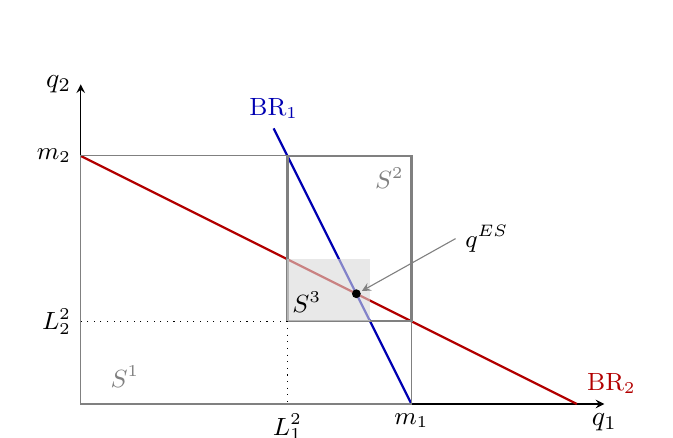
\begin{tikzpicture}[scale=7,>=stealth]
  \draw[->] (0,0) -- (0.95,0) node[below] {$q_1$};
  \draw[->] (0,0) -- (0,0.58) node[left] {$q_2$};
  \draw[thick,blue!70!black] (0.6,0) -- (0.35,0.5) node[above] {\small $\mathrm{BR}_1$};
  \draw[thick,red!70!black] (0,0.45) -- (0.9,0) node[above right] {\small $\mathrm{BR}_2$};
  \draw[gray] (0,0) rectangle (0.6,0.45);
  \draw[gray,thick] (0.375,0.15) rectangle (0.6,0.45);
  \fill[gray!30,opacity=0.6] (0.375,0.15) rectangle (0.525,0.2625);
  \node[gray] at (0.08,0.05) {\small $S^1$};
  \node[gray] at (0.56,0.41) {\small $S^2$};
  \node at (0.41,0.185) {\small $S^3$};
  \fill (0.5,0.2) circle (0.008);
  \draw[gray,->] (0.68,0.3) node[right,black] {\small $q^{ES}$} -- (0.51,0.205);
  \node[below] at (0.6,0) {\small $m_1$};
  \node[left] at (0,0.45) {\small $m_2$};
  \draw[dotted] (0.375,0.15) -- (0.375,0) node[below] {\small $L_1^2$};
  \draw[dotted] (0.375,0.15) -- (0,0.15) node[left] {\small $L_2^2$};
\end{tikzpicture}
\end{center}
\refbib{Tadelis (2013) \S4.2.2, Figure 4.1, p.~67; Gibbons (1992) \S1.2.A, Figure 1.2.2, pp.~19--20.}
\rubrica{
\item Width contraction and convergence to a fixed point: 1 pt.
\item Interior closed form: 0.5 pt; corner case with its condition: 0.5 pt.
\item No finite singleton (exact halving): 0.25 pt.
\item Graph: axes 0.15, both best replies with correct intercept order 0.25, nested rectangles 0.25,
  $q^{ES}$ at the crossing 0.1. Corner case omitted: max.\ 2 pts.
}
\end{sol}

\textbf{d)} (3 points) Now $n\ge3$ identical firms, each with marginal cost $c\in(0,a)$. Characterize
$S^\infty$ and quantify the range of industry output and of the market price compatible with IESDS;
compare with $n=2$.
\resolespaco
\begin{sol}
\passo{round 1}{The argument of a) holds with $Q_{-i}\equiv\sum_{j\ne i}q_j\ge0$ in place of $q_j$:
$S_i^1=[0,m]$, $m=\tfrac{a-c}{2b}$.}
\passo{round 2 removes nothing}{With every rival in $[0,m]$, $Q_{-i}$ ranges over
$[0,(n-1)m]\supseteq[0,2m]=[0,(a-c)/b]$ because $n-1\ge2$. Each $q\in[0,m]$ is the unique maximizer
against $Q_{-i}=(a-c)/b-2q\in[0,(a-c)/b]$, which rivals can produce (e.g.\ equal quantities
$Q_{-i}/(n-1)\le m$). So $S^2=S^1$, and $S^\infty=[0,m]^n$.}
\passo{range}{$Q\in\big[0,\tfrac{n(a-c)}{2b}\big]$ and $P\in\big[\max\{0,a-\tfrac{n(a-c)}2\},\,a\big]$.
The set contains zero output ($P=a$), the monopoly output (one firm at $m$), the competitive output
$(a-c)/b$ (two firms at $m$), and outputs above it ($P<c$). For $n=2$:
$Q^{ES}=\tfrac{2(a-c)}{3b}$, $P^{ES}=\tfrac{a+2c}3$, a single point.}
\intuicao{With two firms, a bound on the rival's output is a bound on everything the firm faces; with
three, two rivals at the top of their range can already flood the market, so no quantity in $[0,m]$
can be ruled out. IESDS exists here but loses uniqueness abruptly at $n=3$.}
\refbib{Gibbons (1992) \S1.2.A, pp.~20--21; Tadelis (2013) \S4.2.3, pp.~67--68.}
\rubrica{
\item Round 1 with $Q_{-i}$: 0.5 pt. Round 2 removes nothing, with the attainability of $Q_{-i}$: 1.25 pts.
\item Output and price ranges with the comparison to $n=2$: 1.25 pts.
\item Duopoly recursion applied to $n\ge3$ (concluding uniqueness): max.\ 1 pt.
}
\end{sol}

\textbf{e)} (3 points) Parameter analysis for the interior duopoly. Prove the sign of the effect of
$a$, $b$, $c_1$, $c_2$ on $q_1^{ES}$, industry output $Q^{ES}$, the price $P^{ES}$ and firm 1's
profit $\pi_1^{ES}$. Tabulate, study $c_1\to c_2$, $c_1\uparrow(a+c_2)/2$ and the move from $n=2$ to
$n=3$, and read the results against the uniqueness and invariance criteria.
\resolespaco
\begin{sol}
\passo{closed forms}{$q_1^{ES}=\tfrac{a-2c_1+c_2}{3b}$, $Q^{ES}=\tfrac{2a-c_1-c_2}{3b}$,
$P^{ES}=a-bQ^{ES}=\tfrac{a+c_1+c_2}3$, and since $P^{ES}-c_1=bq_1^{ES}$,
$\pi_1^{ES}=b(q_1^{ES})^2=\tfrac{(a-2c_1+c_2)^2}{9b}$.}
\passo{signs}{Differentiating: $\partial_aq_1=\tfrac1{3b}$, $\partial_{c_1}q_1=-\tfrac2{3b}$,
$\partial_{c_2}q_1=\tfrac1{3b}$, $\partial_bq_1=-q_1/b$; $Q$: $+a$, $-c_1$, $-c_2$, $-b$;
$P$: $\tfrac13$ in $a$, $c_1$, $c_2$, and $0$ in $b$; $\pi_1=b q_1^2$ has the signs of $q_1$ in
$a,c_1,c_2$ and $\partial_b\pi_1=-\pi_1/b<0$.}
\begin{center}
\begin{tabular}{lcccc}\toprule
 & $a$ & $b$ & $c_1$ & $c_2$\\\midrule
$q_1^{ES}$ & $+$ & $-$ & $-$ & $+$\\
$Q^{ES}$ & $+$ & $-$ & $-$ & $-$\\
$P^{ES}$ & $+$ & $0$ & $+$ & $+$\\
$\pi_1^{ES}$ & $+$ & $-$ & $-$ & $+$\\\bottomrule
\end{tabular}
\end{center}
\passo{limits}{$c_1\to c_2=c$: $q_i^{ES}=\tfrac{a-c}{3b}$, the symmetric case of the textbooks.
$c_1\uparrow(a+c_2)/2$: $q_1^{ES}\to0$ and $q_2^{ES}\to m_2$, matching the corner of c)
continuously. $n=2\to3$: the prediction jumps from a point to the box $[0,m]^3$ (d).}
\passo{reading}{A rival's cost increase helps a firm; one third of any cost change passes to the price.
In costs and demand, the IESDS prediction is invariant (continuous, even through the exit threshold);
in the number of firms it fails the uniqueness criterion abruptly. The speed of convergence (width
halves each round) does not depend on any parameter.}
\rubrica{
\item Closed forms incl.\ $\pi_1=bq_1^2$: 0.5 pt. Signs proved: 1.25 pts.
\item Table 0.25 pt; limits 0.5 pt; reading against the criteria 0.5 pt.
\item Signs without derivation or without reading: max.\ half the item.
}
\end{sol}

% =============================================================================
\bloco{3}{Integrative: spatial competition}{Lecture 1 \,\textbullet\, 25 points}

\noindent\emph{Common setting for Questions 5 and 6.} Along a stretch of highway in the interior of
São Paulo state, $n\ge2$ towns are equally spaced (distance $1$ between neighbours) and numbered
$1,\dots,n$; unless stated otherwise each town has one unit of households. Two fuel-retail chains, $A$
and $B$, simultaneously choose one town each in which to open a single station (both may choose the
same town). Prices and products are identical and fixed. Every household refuels at the nearest
station, measured along the highway, and splits evenly if both are equally distant. Each chain
maximizes the number of households it serves. A household's travel cost is its distance to the station
it uses; total travel distance is the sum over households.

\questao{(10 points) Objective items.}

\textbf{a)} (3 points) \emph{Normal form $\times$ IESDS $\times$ welfare.} Suppose instead that the
$n\ge3$ towns are equally spaced around a ring road (like the Rodoanel around São Paulo), with
distance measured along the ring. Which statement is correct?
\begin{alternativas}
\item A chain serves more households the farther it is from its rival, so IESDS selects antipodal pairs, which also minimize total travel distance.
\item As on a straight highway, IESDS makes the chains cluster in a single town, a profile that maximizes total travel distance.
\item Every profile gives each chain $n/2$ households, IESDS eliminates nothing, and an antipodal pair of stations minimizes total travel distance.
\item Every profile gives each chain $n/2$ households, IESDS eliminates nothing, and total travel distance is the same in every profile.
\item Every profile gives each chain $n/2$ households, so every town is a strictly dominant strategy and every profile is a strict dominant-strategy equilibrium.
\end{alternativas}
\gabarito{C}
\begin{sol}
\passo{payoffs}{Same town: $n/2$ each. Otherwise, at ring distance $g$, the two arcs hold $g-1$ and
$n-g-1$ interior towns, each split evenly by its midpoint: $u_A=1+\tfrac{g-1}2+\tfrac{n-g-1}2=\tfrac n2$.}
\passo{IESDS}{All payoffs are equal, so no strategy is strictly (or weakly) dominated: $S^\infty=S$.
Nor is any strategy strictly dominant (E), and no location pattern is selected (A, B).}
\passo{welfare}{An arc with $t$ interior towns between two stations costs
$\sum_{s=1}^t\min\{s,t+1-s\}=\lfloor(t+1)^2/4\rfloor$, so gap $g$ costs
$f(g)=\lfloor g^2/4\rfloor+\lfloor(n-g)^2/4\rfloor$ ($g=0$: $\lfloor n^2/4\rfloor$). Using
$\lfloor(t+1)^2/4\rfloor-\lfloor t^2/4\rfloor=\lfloor(t+1)/2\rfloor$,
$f(g+1)-f(g)=\lfloor\tfrac{g+1}2\rfloor-\lfloor\tfrac{n-g}2\rfloor\le0$ for $g\le\tfrac{n-1}2$: the
antipodal gap $\lfloor n/2\rfloor$ minimizes (D false), clustering maximizes.}
\refbib{Lecture 1, ``Application: spatial competition''; Tadelis (2013) \S4.2.3, p.~67.}
\end{sol}

\medskip
\textbf{b)} (3 points) \emph{IESDS $\times$ non-uniform population.} Back on the straight highway,
let $n$ be odd and let town $1$, a regional capital, have $1+2h$ households, with
$h\in\{1,\dots,(n-1)/2\}$; every other town keeps one. IESDS selects:
\begin{alternativas}
\item the median town $(n+1)/2$ for both chains, since IESDS depends only on the number of towns
\item town $(n+1)/2-h$ for both chains
\item town $(n+1)/2-2h$ for both chains
\item towns $(n+1)/2-h$ and $(n+1)/2-h+1$ for each chain
\item town $1$, the capital, for both chains, for every $h\ge1$
\end{alternativas}
\gabarito{B}
\begin{sol}
\passo{elimination rule}{Let $T=n+2h$ be total population and $W(\le\ell)$ the population of towns
$1,\dots,\ell$. In a reduced game with towns $\{\ell,\dots,r\}$ for both chains, $\ell$ is strictly
dominated by $\ell+1$ iff $W(\le\ell)<T/2$: against $s\ge\ell+2$ moving inward shifts the boundary
by half a town and always gains; against $s=\ell+1$ it compares $W(\le\ell)$ with $T/2$; against
$s=\ell$ it compares $T/2$ with $T-W(\le\ell)$. Symmetrically on the right.}
\passo{survivor}{IESDS stops at the weighted median: $W(\le m)=2h+m\ge T/2\iff m\ge\tfrac{n+1}2-h-\tfrac12$,
and $W(\ge m)=n-m+1\ge T/2\iff m\le\tfrac{n+1}2-h+\tfrac12$. With $n$ odd, the unique integer is
$m^*=(n+1)/2-h$.}
\passo{distractors}{A ignores the weights; C shifts by the extra households $2h$ instead of half of
them; D treats total population as even (two medians); E confuses the largest town with the median.}
\refbib{Tadelis (2013) \S4.2.1, pp.~63--65; Lecture 1, ``Application: spatial competition''.}
\end{sol}

\medskip
\textbf{c)} (2 points, T or F) \emph{Dominance $\times$ IESDS.} With uniform population and any odd
$n\ge3$, the median town is a strictly dominant strategy for each chain, which is why IESDS selects it.
\gabarito{F}
\begin{sol}
\passo{n = 3}{True only here: town 2 earns $2$ against a rival at an end and $3/2$ against a rival at
2, strictly more than any end town in each case.}
\passo{n >= 5}{Against $s_B=1$: $u_A(2,1)=n-1$, while $u_A\big(\tfrac{n+1}2,1\big)=n-\tfrac{n+1}4<n-1$
for $n>3$. The median is not even optimal against every rival location; IESDS selects it only after
$(n-1)/2$ rounds, using common knowledge of rationality, not rationality alone.}
\refbib{Lecture 1, ``Iterated elimination of dominated strategies''; Tadelis (2013) \S4.1.2, p.~61.}
\end{sol}

\medskip
\textbf{d)} (2 points, T or F) \emph{Dominance $\times$ policy.} Let $n\ge4$ be even. A municipal
licensing rule allows chain $A$ only in towns $1,\dots,n/2$ and chain $B$ only in towns
$n/2+1,\dots,n$. Then each chain has a strictly dominant strategy, and the two stations end up in
adjacent towns at the centre of the highway.
\gabarito{T}
\begin{sol}
\passo{proof}{Now $s_A<s_B$ always, so $u_A=(s_A+s_B-1)/2$, strictly increasing in $s_A$ for every
$s_B$: $s_A=n/2$ is strictly dominant. $u_B=n-u_A$ is strictly decreasing in $s_B$: $s_B=n/2+1$.
Total travel distance is $n(n-2)/4$, against the optimum $\lfloor n^2/8\rfloor$ of Question 6 d), a
ratio that tends to $2$: zoning by halves does not undo the clustering.}
\refbib{Tadelis (2013) \S4.1.2, p.~61; Lecture 1, ``Application: spatial competition''.}
\end{sol}

% -----------------------------------------------------------------------------
\questao{(15 points) \emph{Integrative: normal form $\times$ dominance and IESDS $\times$ Pareto
optimality $\times$ solution-concept criteria (existence, uniqueness, invariance).} Use the common
setting above, with uniform population.}

\textbf{a)} (3 points) Write the game in normal form for a general $n$, with each chain's payoff in
closed form, and prove that it is constant-sum. Deduce which location profiles are Pareto optimal for
the two chains. Who, then, can be harmed by the chains' choices?
\resolespaco
\begin{sol}
\passo{normal form}{$I=\{A,B\}$, $S_A=S_B=\{1,\dots,n\}$. If $s_A<s_B$: $A$ serves towns
$1,\dots,s_A$ and half of the $s_B-s_A-1$ towns strictly between (the midpoint town, if any, is split),
so $u_A=s_A+\tfrac{s_B-s_A-1}2=\tfrac{s_A+s_B-1}2$. If $s_A=s_B$: $u_A=\tfrac n2$. If $s_A>s_B$:
$u_A=(n-s_A+1)+\tfrac{s_A-s_B-1}2=n-\tfrac{s_A+s_B-1}2$. $u_B$ follows by symmetry.}
\passo{constant sum}{Every household is served by exactly one chain (or split in halves), so
$u_A+u_B=n$ for every profile; the formulas confirm it case by case.}
\passo{Pareto}{If $u_A$ rises, $u_B$ falls by the same amount: no profile Pareto dominates another, so
\emph{every} profile is Pareto optimal for the chains. The only parties whose welfare differs across
profiles are the households, through travel distance, which no chain internalizes.}
\refbib{Tadelis (2013) \S3.1, pp.~46--49; \S3.3.3, p.~56; Lecture 1, ``Dominance and social dilemmas''.}
\rubrica{
\item Three-case payoff with the midpoint split: 1.25 pts (a case missing: $-0.5$ pt each).
\item Constant sum: 0.5 pt. Every profile Pareto optimal for the chains: 0.75 pt.
\item Households identified as the harmed party: 0.5 pt.
\item ``The IESDS profile is Pareto inefficient for the chains'': 0 for the Pareto line.
}
\end{sol}

\textbf{b)} (3 points) Characterize $S^\infty$ for every $n\ge2$: which towns are eliminated in each
round, how many rounds there are, and which profiles survive, separately for odd and even $n$. Prove
your characterization. What order of knowledge of rationality does the prediction require?
\resolespaco
\begin{sol}
\passo{claim}{Round $k$ removes towns $k$ and $n+1-k$ for both chains, as long as at least three towns
remain. After $k$ rounds the set is $\{k+1,\dots,n-k\}$.}
\passo{extremes dominated}{Let the current set be $\{\ell,\dots,r\}$, $r=n+1-\ell$, $r-\ell\ge2$ (so
$\ell<n/2$). Compare $\ell$ with $\ell+1$: against $s_B=\ell$, $n/2<n-\ell$; against $s_B=\ell+1$,
$\ell<n/2$; against $s_B\ge\ell+2$, $\tfrac{\ell+s_B-1}2<\tfrac{\ell+s_B}2$. So $\ell$ is strictly
dominated by $\ell+1$, and $r$ by $r-1$ by symmetry.}
\passo{interior survives}{A strategy that is optimal against some rival location in the current set
cannot be strictly dominated. For $\ell<s<n/2$: against $s_B=s-1$, locating at $s$ earns $n-s+1>n/2$,
more than any other town, so $s$ is optimal; symmetrically on the right. The central town(s) are
optimal against the rival at the centre: odd $n$, $(n+1)/2$ earns $n/2>(n-1)/2$; even $n$, $n/2$ and
$n/2+1$ both earn $n/2$ against $n/2+1$.}
\passo{result}{Odd $n$: after $(n-1)/2$ rounds, $S^\infty=\{(\tfrac{n+1}2,\tfrac{n+1}2)\}$. Even
$n\ge4$: after $n/2-1$ rounds, $S^\infty=\{\tfrac n2,\tfrac n2+1\}^2$ (four profiles, each giving $n/2$
to each chain). $n=2$: every payoff is $1$, nothing is removed. Rounds: $\lceil n/2\rceil-1$.}
\passo{knowledge}{The last round needs $(\lceil n/2\rceil-2)$-th order mutual knowledge of
rationality: the longer the highway, the deeper the reasoning the prediction relies on.}
\refbib{Tadelis (2013) \S4.2.1, pp.~63--65; related exercise: Tadelis Exercise 4.10, p.~78.}
\rubrica{
\item Extreme dominated by its neighbour, all three cases: 1 pt.
\item Interior and central towns survive (optimality argument): 0.75 pt.
\item Survivors and number of rounds for both parities and $n=2$: 0.75 pt. Knowledge order: 0.5 pt.
\item Pattern read off small cases without proof: max.\ a third of the item.
}
\end{sol}

\textbf{c)} (3 points) Replace the towns by a continuum: households are uniformly distributed on
$[0,1]$ (unit mass) and each chain locates anywhere in $[0,1]$. Characterize $S^\infty$. Compare with
b) as the spacing between towns shrinks, and evaluate IESDS against the existence, uniqueness and
invariance criteria.
\resolespaco
\begin{sol}
\passo{payoffs}{$u_A(a,b)=\tfrac{a+b}2$ if $a<b$, $\tfrac12$ if $a=b$, $1-\tfrac{a+b}2$ if $a>b$.}
\passo{endpoints removed}{$0$ is strictly dominated by every $a'\in(0,\tfrac23]$: for $b>a'$,
$\tfrac{a'+b}2>\tfrac b2$; $b=a'$: $\tfrac12>\tfrac{a'}2$; $0<b<a'$: $1-\tfrac{a'+b}2>\tfrac b2\iff
b<1-\tfrac{a'}2$, true for all $b<a'$ iff $a'\le\tfrac23$; $b=0$: $1-\tfrac{a'}2>\tfrac12$. By symmetry
$1$ is removed: $S_i^1=(0,1)$.}
\passo{nothing else}{Take $a\in(0,\tfrac12]$ and any $a'\ne a$. If $a'>a$, against $b=a/2$:
$u_A(a',b)=1-\tfrac{a'+b}2<1-\tfrac{a+b}2=u_A(a,b)$. If $a'<a$, against $b=\tfrac{a+a'}2$:
$u_A(a',b)=\tfrac{a'+b}2\le1-\tfrac{a+b}2=u_A(a,b)\iff a+a'\le1$, true. Both witnesses lie in
$(0,1)$, so no $a'$ strictly dominates $a$ in any round; $a>\tfrac12$ by symmetry. Hence
$S^\infty=(0,1)^2$.}
\passo{comparison}{With $n$ towns the prediction is the centre after $\lceil n/2\rceil-1$ rounds, for
every $n$; in the continuum IESDS removes only the endpoints. The discrete argument relies on a
``next town inward'' with no rival location strictly between; in the continuum there is always one,
where the inward move loses. Existence holds in both; uniqueness is lost in the continuum; and the
prediction is not invariant to how finely locations are modelled, since the limit of the discrete
predictions is not the prediction of the limit game.}
\refbib{Tadelis (2013) \S3.3.2, pp.~55--56; \S4.2.3, pp.~67--68; Cabral (2017) Ch.~14,
``Horizontal differentiation'', pp.~357--358.}
\rubrica{
\item Payoff function: 0.5 pt. Endpoints strictly dominated (with an explicit dominator): 0.75 pt.
\item No other strategy dominated, with explicit witnesses for both $a'>a$ and $a'<a$: 1 pt.
\item Comparison and the three criteria: 0.75 pt.
\item Concluding $S^\infty=\{(\tfrac12,\tfrac12)\}$ by analogy with b): max.\ 1 pt.
}
\end{sol}

\textbf{d)} (3 points) Welfare. Find the minimum total travel distance $D^{\min}(n)$ over all location
pairs and the total travel distance $D^{ES}(n)$ at the IESDS survivors. Prove that
$D^{ES}/D^{\min}=2$ for every odd $n\ge3$, and characterize the ratio for even $n$. For the
continuum version, draw each household's travel distance as a function of its location when (i) both
stations are at $\tfrac12$ and (ii) the stations are at $\tfrac14$ and $\tfrac34$, and read the totals
off the figure.
\resolespaco
\begin{sol}
\passo{optimum}{Given stations $x<y$, households left of the midpoint use $x$: an optimum splits the
towns into a left block of $t$ and a right block of $n-t$, each served from its median. A block of $t$
towns served from its median costs $\lfloor t^2/4\rfloor$. Minimizing
$\lfloor t^2/4\rfloor+\lfloor(n-t)^2/4\rfloor$ (same difference argument as Question 5 a) gives
$t=\lfloor n/2\rfloor$ and $D^{\min}(n)=\lfloor n^2/8\rfloor$.}
\passo{IESDS}{Odd $n$: both at the median, $D^{ES}=2\sum_{s=1}^{(n-1)/2}s=\tfrac{n^2-1}4$. Even $n$:
both in one central town, $\tfrac{n^2}4$; in the adjacent central pair, $\tfrac{n(n-2)}4$.}
\passo{ratio}{Odd $n$: $n^2\equiv1\pmod 8$, so $\lfloor n^2/8\rfloor=\tfrac{n^2-1}8$ and the ratio is
exactly $2$. Even $n$, $4\mid n$: $D^{\min}=\tfrac{n^2}8$, ratio $\in\{\tfrac{2(n-2)}n,\,2\}$.
$n\equiv2\pmod4$: $D^{\min}=\tfrac{n^2-4}8$, ratio $\in\{\tfrac{2n}{n+2},\,\tfrac{2n^2}{n^2-4}\}$, the
second above $2$ (e.g.\ $\tfrac94$ at $n=6$).}
\passo{continuum figure}{Case (i) is the V-shaped $|x-\tfrac12|$, area $\tfrac14$; case (ii) is the
W-shaped $\min\{|x-\tfrac14|,|x-\tfrac34|\}$, area $\tfrac18$: ratio $2$, as in the odd discrete case.}
\begin{center}
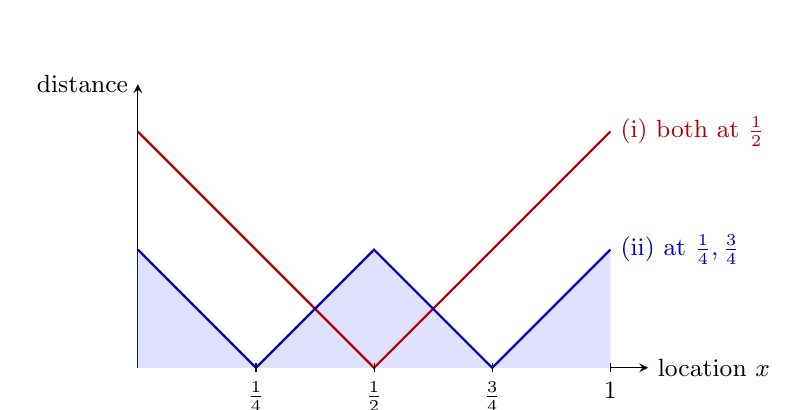
\begin{tikzpicture}[scale=6,>=stealth]
  \draw[->] (0,0) -- (1.08,0) node[right] {\small location $x$};
  \draw[->] (0,0) -- (0,0.6) node[left] {\small distance};
  \fill[blue!12] (0,0.25) -- (0.25,0) -- (0.5,0.25) -- (0.75,0) -- (1,0.25) -- (1,0) -- (0,0) -- cycle;
  \draw[thick,red!70!black] (0,0.5) -- (0.5,0) -- (1,0.5) node[right] {\small (i) both at $\tfrac12$};
  \draw[thick,blue!70!black] (0,0.25) -- (0.25,0) -- (0.5,0.25) -- (0.75,0) -- (1,0.25) node[right] {\small (ii) at $\tfrac14,\tfrac34$};
  \foreach \t/\l in {0.25/\tfrac14,0.5/\tfrac12,0.75/\tfrac34,1/1} \draw (\t,0.01) -- (\t,-0.01) node[below] {\small $\l$};
\end{tikzpicture}
\end{center}
\intuicao{Each chain moves inward to steal households from the rival; the households pay for it in
kilometres, and the chains, playing a constant-sum game, are indifferent to that cost.}
\refbib{Lecture 1, ``Application: spatial competition''; Cabral (2017) Ch.~14, pp.~357--358.}
\rubrica{
\item $D^{\min}=\lfloor n^2/8\rfloor$ with the block argument: 1 pt.
\item $D^{ES}$ for both parities: 0.5 pt. Ratio $2$ for odd $n$ proved: 0.5 pt; even case: 0.25 pt.
\item Figure: axes 0.25, both curves with kinks at the station sites 0.25, areas read 0.25.
\item Optimum guessed at the quartile towns for every $n$ without the block argument: max.\ 1.5 pts.
}
\end{sol}

\textbf{e)} (3 points) Parameter analysis. Let towns be $d>0$ apart and hold $N>0$ households each.
Prove how $n$, $d$ and $N$ affect the number of IESDS rounds $K$, the IESDS and minimum travel
distance per household, and their ratio. Tabulate, study $n=2$ and $n\to\infty$ (in units of the
stretch length $d(n-1)$), and give the economic and policy reading.
\resolespaco
\begin{sol}
\passo{scaling}{Distances scale with $d$ and the number of households with $N$; the game's payoffs
are multiplied by $N$, which leaves every dominance relation and so $K$ and $S^\infty$ unchanged:
$K=\lceil n/2\rceil-1$ depends on $n$ only. Per household (odd $n$):
$\bar D^{ES}=d\,\tfrac{n^2-1}{4n}$ and $\bar D^{\min}=d\,\tfrac{\lfloor n^2/8\rfloor}{n}$, both
increasing in $n$ and in $d$, neither depending on $N$; the ratio depends on $n$ only.}
\begin{center}
\begin{tabular}{lccc}\toprule
 & $n$ & $d$ & $N$\\\midrule
$K$ & $+$ (weakly) & $0$ & $0$\\
$\bar D^{ES}$, $\bar D^{\min}$ & $+$ & $+$ & $0$\\
$D^{ES}/D^{\min}$ & $2$ (odd); $\to2$ (even) & $0$ & $0$\\\bottomrule
\end{tabular}
\end{center}
\passo{limits}{$n=2$: no strategy is removed; the survivors include both the optimum (one station per
town, distance $0$) and clustering ($Nd$): IESDS has no bite. $n\to\infty$: relative to the stretch
length, $\bar D^{ES}/(d(n-1))\to\tfrac14$ and $\bar D^{\min}/(d(n-1))\to\tfrac18$; both even-$n$ ratios
tend to $2$.}
\passo{reading}{Clustering at the centre doubles the travel cost, whatever the size of the towns or
the distance between them. The chains do not care (constant sum), so the inefficiency is not a social
dilemma among the players but an externality on households. A licensing rule by halves keeps the
stations adjacent (Question 5 d); restoring the optimum needs the planner to fix both sites. Brazilian
law rules out the bluntest instrument, municipal bans on same-sector stores in an area (STF,
\emph{Súmula Vinculante} 49: ``Ofende o princípio da livre concorrência lei municipal que impede a
instalação de estabelecimentos comerciais do mesmo ramo em determinada área'').}
\rubrica{
\item Invariance of $K$ and $S^\infty$ to $N$ and $d$ argued: 0.75 pt. Per-household signs: 0.75 pt.
\item Table 0.25 pt; limits 0.5 pt; reading (players vs households, policy) 0.75 pt.
\item Signs without proof or reading: max.\ half the item.
}
\end{sol}

\end{document}
